\documentclass[12pt]{article}
% format
% \usepackage[a4paper, total={6in, 9in}]{geometry}                         

% math symbols
\usepackage{amsmath}
\usepackage{amsthm}
\usepackage{amssymb}
\usepackage[shortlabels]{enumitem} 
\usepackage{mathtools}
\usepackage{bbm}

% annotations
\setlength{\marginparwidth}{2cm}
\usepackage{soul}
\usepackage{pdfcomment}

% figures
\usepackage{graphicx}
\usepackage{subcaption}

% theorems
\theoremstyle{definition}
\newtheorem{thm}{Theorem}
\newtheorem{prop}[thm]{Proposition}
\newtheorem{lemma}[thm]{Lemma}
\newtheorem{rmk}[thm]{Remark}
\newtheorem{defn}[thm]{Definition}
\newtheorem{cor}[thm]{Corollary}
\newtheorem{exo}[thm]{Exercise}
\newtheorem{fact}[thm]{Fact}

% definition equal
\newcommand{\defeq}{\vcentcolon=}
\newcommand{\eqdef}{=\vcentcolon}
\pdfcommentsetup{color=yellow, opacity=0.5}

% bibliography
\usepackage[backend=biber,style=alphabetic, sorting=ynt]{biblatex}
\bibliography{ref}

% url highlight
\usepackage{hyperref}

% algos
\usepackage[linesnumbered,ruled,vlined]{algorithm2e}
\SetArgSty{textnormal}

% bullet point style
% \renewcommand{\labelitemi}{\tiny$\blacksquare$}

% new commands
\DeclareMathOperator{\dom}{dom}
\DeclareMathOperator{\Hess}{\textbf{H}}
\DeclareMathOperator{\Diag}{Diag}
\DeclareMathOperator{\Tr}{Tr}
\DeclareMathOperator{\ind}{i}
\DeclareMathOperator{\sgn}{sign}

% figures
\usepackage{tikz}
\usepackage{caption}

% colors
\definecolor{azure}{RGB}{41, 50, 65}
\definecolor{orange}{RGB}{238, 108, 77}
\definecolor{lightblue}{RGB}{224, 251, 252}
\definecolor{blue}{RGB}{152, 193, 217}
\definecolor{darkblue}{RGB}{61, 90, 128}
\definecolor{green}{RGB}{67, 170, 139}
\definecolor{purple}{RGB}{199, 125, 255}

\begin{document}
    \section{Finding \texorpdfstring{$k$}{k}-chords in half graphs}
    
    The aim of this section 
    is to prove the following 
    proposition.

    \begin{prop} \label{prop:hg}
        For any $k \neq 1, 4$,
        there exists $n \in \mathbb{N}$
        such that the half
        graph $H_{n}$ 
        contains an induced 
        $k$-chord.
    \end{prop}

    Before tackling the
    above statement, we notice the
    following fact.
    
    \begin{fact} \label{fact:edges}
        For any graph $G$
        and cycle $C$ in $G$, 
        the number of chords in $C$ 
        is given by $e\left(G\left[V\left(C\right)\right]\right)
        - \left|C\right|$.
    \end{fact}
    
    We now establish 
    some notation. For
    any half graph $H_{n}$ 
    with $n \geq 3$, label
    its vertices as follows.
    \begin{figure}[h]
        \centering
        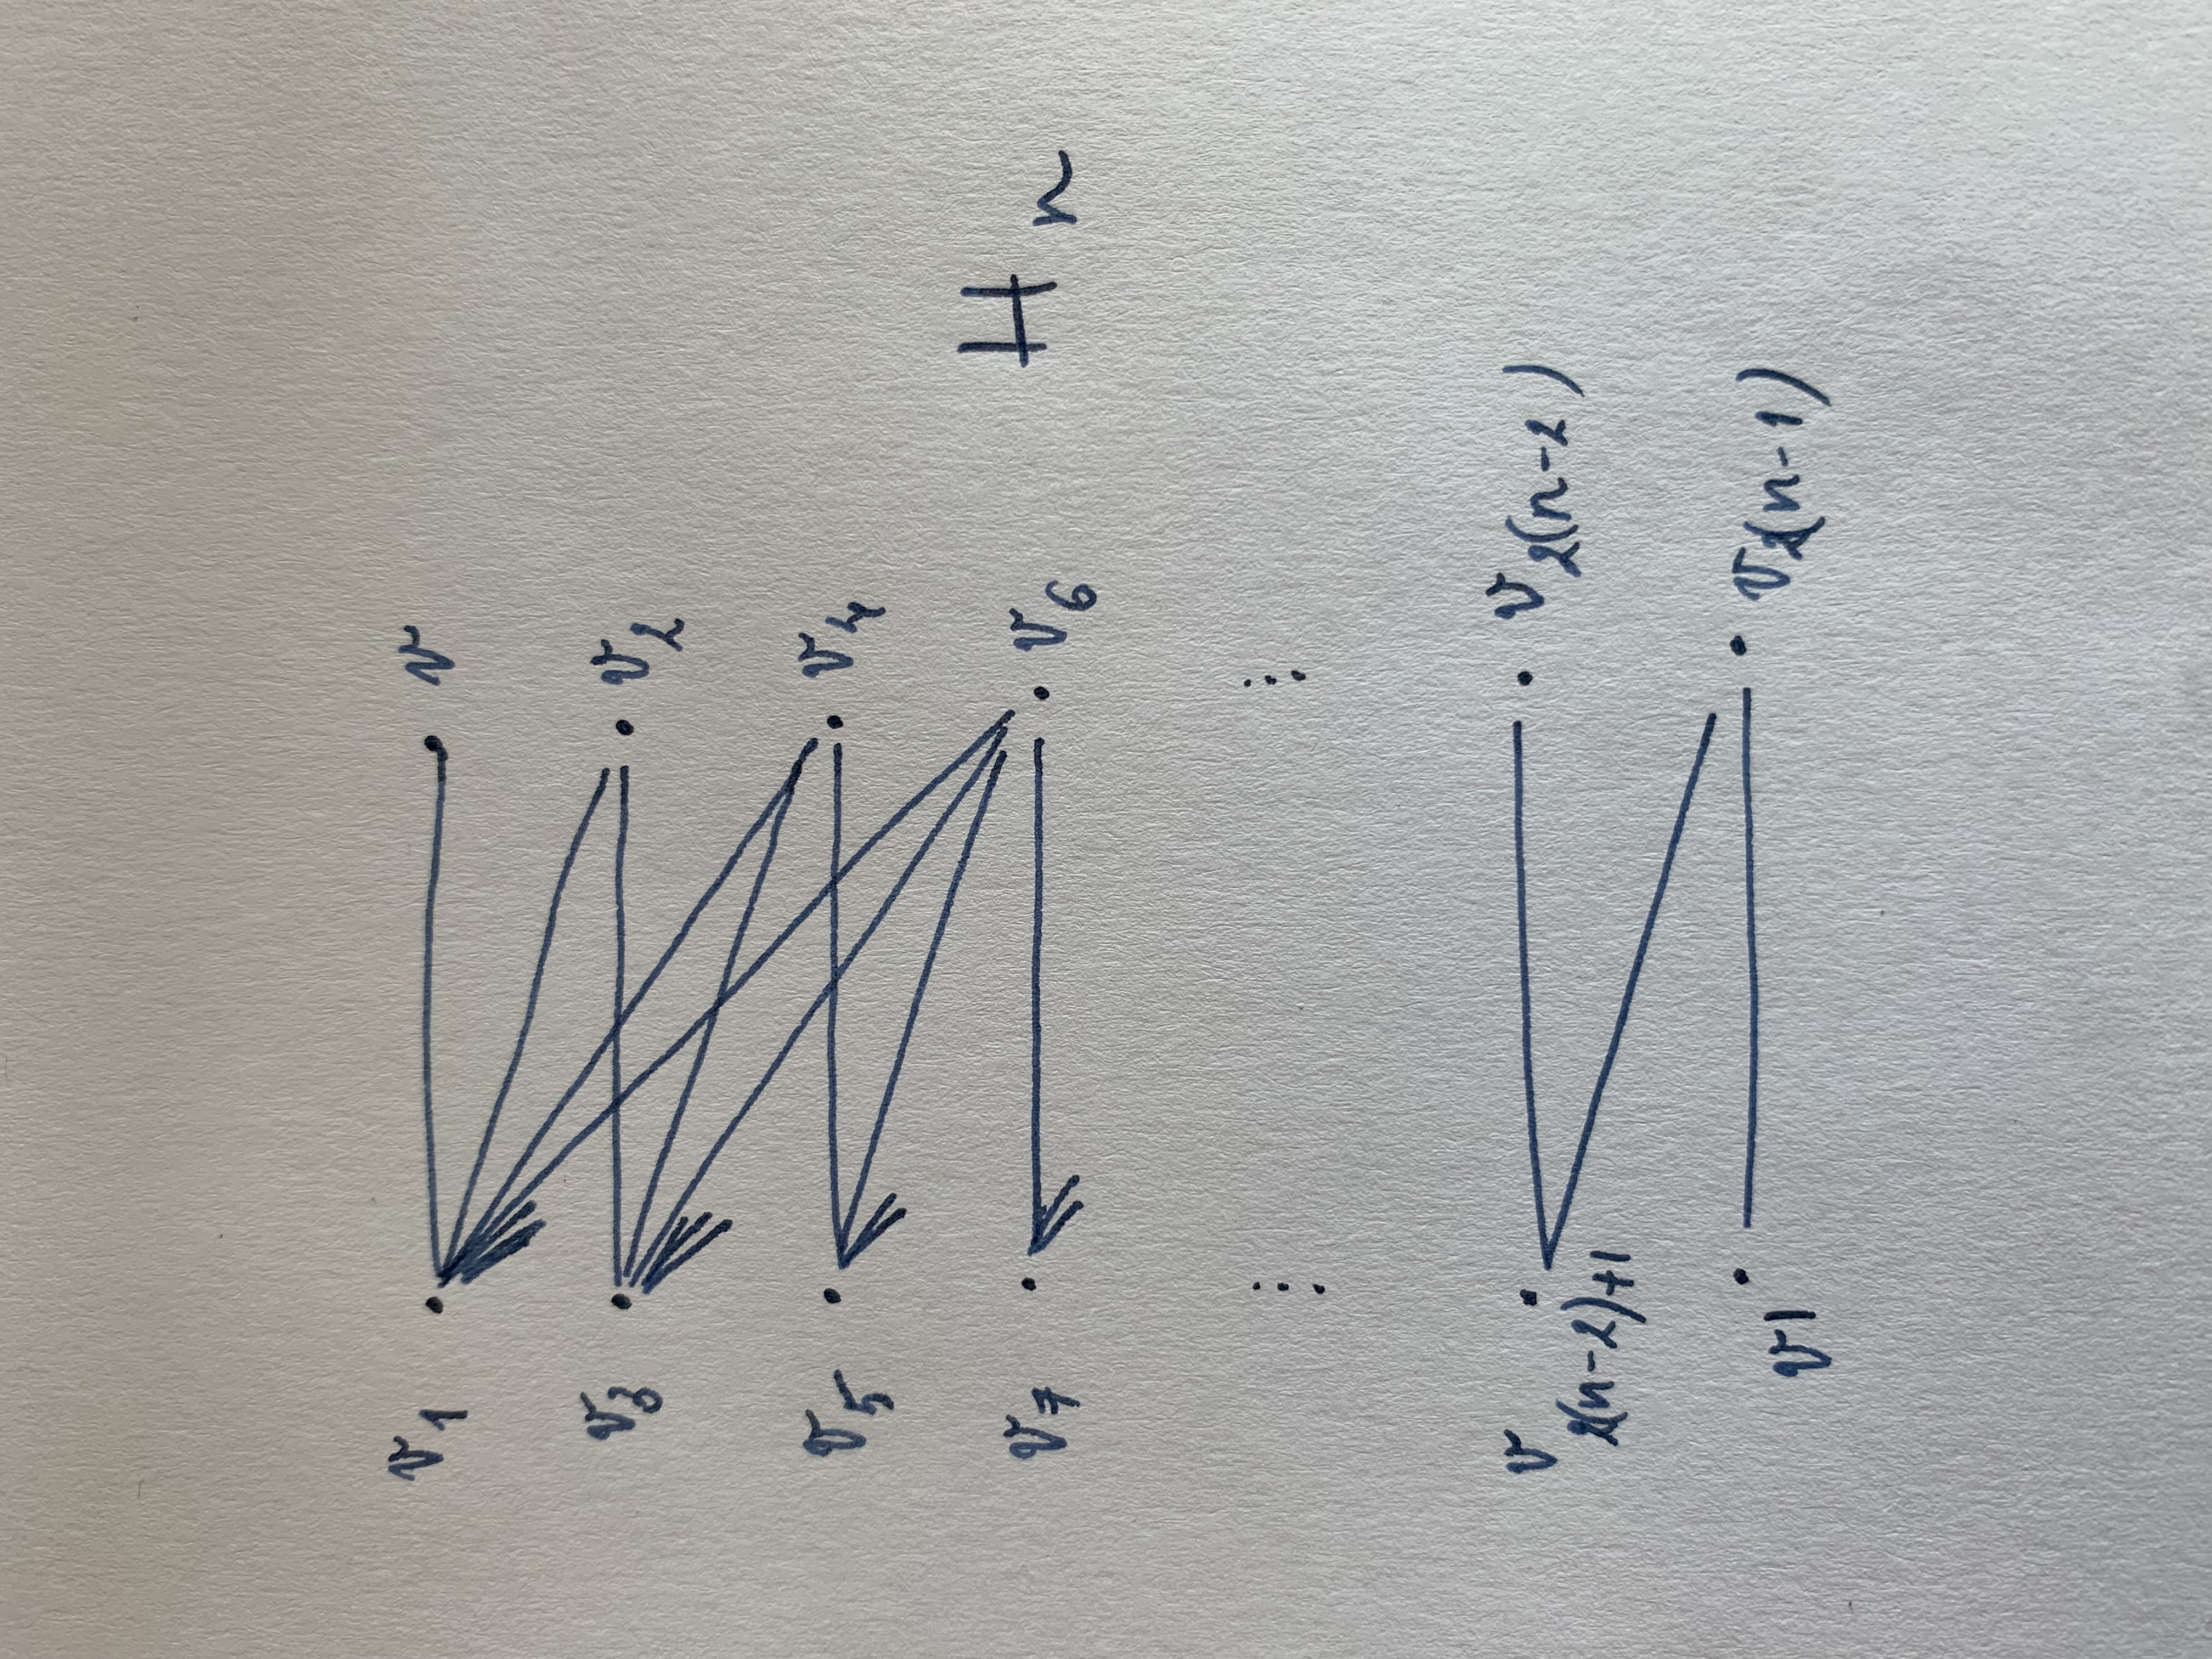
\includegraphics[width=0.35\linewidth, angle=270]{Figure_k-chord.jpg}
        \caption{Vertex labeling of a half graph}
        \label{fig:hg}
    \end{figure}

    Notice that the cycle
    $\left(v_1, v_2, \ldots,
    v_{2\left(n-1\right)}, v_1\right)$ 
    induces a $k$-chord
    $C_{n}$ in $H_{n}$
    with the number $K_{n}$ 
    of chords being (by Fact \ref{fact:edges}):
    \begin{gather*}
        K_{n} = \left(
        2 + 3 + \cdots + \left(n-1\right)
        + \left(n-1\right)\right)
        -2\left(n-1\right) =
        \frac{n\left(n-3\right)}{2}.
    \end{gather*}
    
    We now notice the following fact
    which will be useful in the next proofs.

    \begin{fact} \label{fact:new}
        Given a $K_{n}$-chord 
        $C_{n}$, one can obtain
        a new $k$-chord by removing
        vertices $v_{2n_1}, 
        v_{2n_2}, \ldots,
        v_{2n_{m}}, v_{2n_1'+1}, 
        v_{2n_2'+1}, \ldots,
        v_{2n_{m}' + 1}$
        such that
        $n_1 < n_2 < \cdots
        < n_{m} < n_1' < n_2'
        < \ldots, n_{m}'$.
        This last condition is
        necessary to ensure that 
        the vertices in $V\left(C_{n}\right)
        \setminus \left\{
        v_{2n_1}, \ldots, 
        v_{2n_{m}},
        v_{2n_1'+1}, \ldots,
        v_{2n_{m}'+1}\right\}$
        are part of a unique cycle.
        The cycle (and the relative
        induced $k$-chord)
        we take into consideration is
        \begin{gather*}
            \left(v_{2i_1 + 1}, 
            v_{2j_1}, \ldots,
            v_{2i_{n-m}+1},
            v_{2j_{n-m}},
            v_{2i_1 + 1}\right),
        \end{gather*}
        where 
        $\left\{i_1, \ldots, i_{n-m}\right\} =
        \left\{1, \ldots, n\right\} \setminus 
        \left\{n_1', \ldots, n_{m}'\right\}$
        and
        $\left\{j_1, \ldots j_{n-m}\right\}
        = \left\{1, \ldots, n\right\}
        \setminus \left\{n_1, \ldots, n_{m}\right\}$ 
        with $i_1 < \cdots < i_{n-m}$
        and
        $j_1 < \cdots < j_{n-m}$.
    \end{fact}
    
    Now, notice that for any
    $n \geq 4$, we have that
    $K_{n} - K_{n-1} = n-2$.
    Our strategy is to find
    and induced $k$-chord
    into $H_{n}$ with
    $K_{n-1} \leq k \leq K_{n}$ 
    for al $k \neq 1,4$.
    The following lemma
    represents a step towards 
    this objective.

    \begin{lemma} \label{lemma:most}
        For any  $n \geq 4$ and
        any $2 \leq l \leq n-2$,
        we have that $C_{n}$ contains an induced
        $\left(K_{n} - l\right)$-chord
        (and thus, so does $H_{n}$).
    \end{lemma}
    \begin{proof}
        Let $q = l-1$. Notice that
        $C_{n}$ has the following
        cycle, obtained from $C_{n}$
        by removing $v_{2q}$ and
        $v_{2\left(n-2\right)+1}$
        as in Fact \ref{fact:new}.
        We have:
        \begin{gather*}
            C_{n}' \defeq
            \left(v_1, v_2, \ldots,
            v_{2\left(q-1\right)+1},
            v_{2\left(q+1\right)}, \ldots ,
            v_{2\left(n-2\right)},
            v_{2\left(n-3\right) + 1},
            v_{2\left(n-1\right)}, v_1\right)
        \end{gather*}
        By Fact \ref{fact:new}, 
        $C_{n}'$ induces a $k$-chord.
        Notice that
        $d\left(v_{2q}\right) = q+1 = l$
        and $d\left(v_{2\left(n-2\right)+1}\right) = 2$.
        Since $\left|C_{n}'\right| = 
        \left|C_{n}\right| - 2$, 
        Fact \ref{fact:edges} tells
        us that the number of 
        chords of $C_{n}'$ is
        \begin{gather*}
            K_{n} - \left(l-2\right) - 2 = K_{n} - l.
        \end{gather*}
        
        This concludes the proof.
    \end{proof}

    Now, notice that $K_{4} = 2$ and $K_{5} = 5$.
    Thus, in order to prove Proposition \ref{prop:hg},
    it suffices to find $n$ such that $H_{n}$ contains
    an induced $\left(K_{m}-1\right)$-chord for
    all $m \geq 6$. We claim that such $n$ is $m+1$.

    \begin{lemma} \label{lemma:remainder}
        For any $m \geq 6$, we have that $C_{m+1}$ contains
        an induced $\left(K_{m} - 1\right)$-chord
        (and thus, so does $H_{m+1}$).
    \end{lemma}
    \begin{proof}
        Consider the $K_{m+1}$-chord $C_{m+1}$.
        Just as in the proof of Lemma \ref{lemma:most},
        consider the $k$-chord $C_{m+1}''$ obtained
        from $C_{m+1}$ by removing the vertices
        $v_2$, $v_{2\left(n-5\right)}$
        $v_{2\left(n-3\right)+1}$, $v_{2\left(n-2\right)+1}$.
        The cycle of $C_{m+1}''$ that
        we will consider is the one
        described in Fact \ref{fact:new}.
        Notice that, since $m \geq 6$, we have
        that all of the above vertices
        are distinct. Moreover, we have
        $d\left(v_2\right) = 2$, 
        $d\left(v_{2\left(n-5\right)}\right) = n-4$,
        $d\left(v_{2\left(n-3\right)+1}\right)=3$,
        $d\left(v_{2\left(n-2\right)+1}\right) = 2$.
        By Fact \ref{fact:edges}, 
        we deduce that the number of chords
        in $C_{m+1}''$ is
        \begin{gather*}
            K_{m+1} - \left(2 + \left(n-4\right)
            + 3 + 2\right) - 4 =
            K_{m+1} - \left(n-1\right) = K_{m} -1.
        \end{gather*}
        This concludes the proof.
    \end{proof}

    As pointed out above, Lemma
    \ref{lemma:most} and \ref{lemma:remainder}
    imply Proposition \ref{prop:hg}.
\end{document}



